\section{遺伝子発現}

DNAは細胞分裂とともに複製される.
またプロモーターと呼ばれる部位にRNApが結合することで,転写が開始される.
転写の結果mRNAができる.
ただし,この転写は転写因子(タンパク質)による制御を受ける.
最後に,mRNAはリボソームでタンパク質に翻訳される.
こうして,遺伝子はタンパク質を発現する.

\begin{figure}[htbp]
  \begin{minipage}[b]{.5\linewidth}
    \centering
    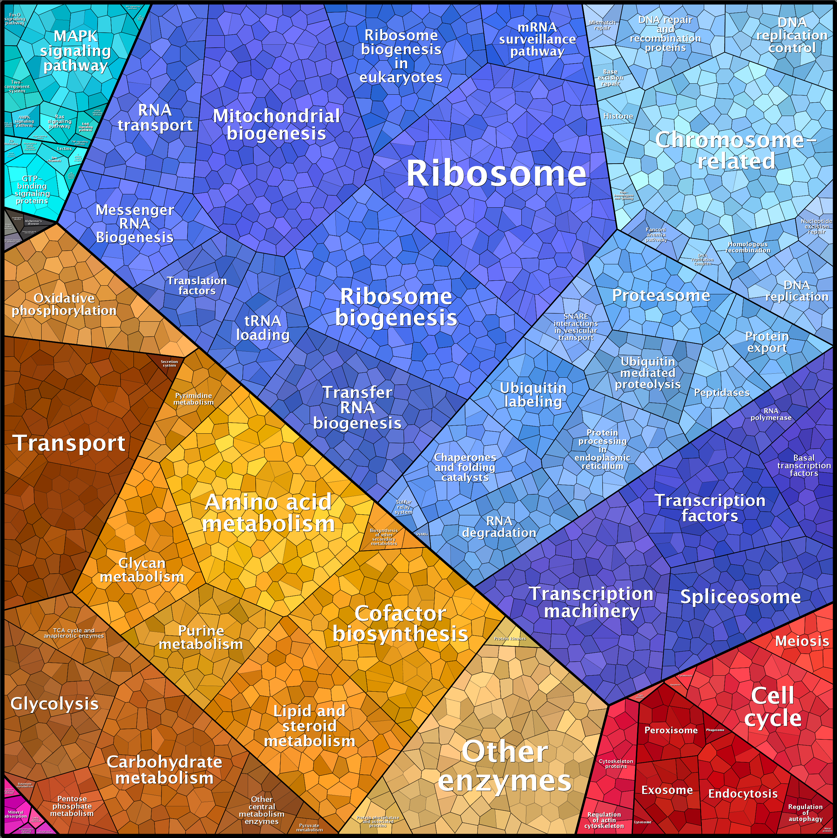
\includegraphics[width=.8\linewidth]{genome.png}
    \subcaption{発現する遺伝子}
    \label{fig:prmap_gen}
  \end{minipage}
  \begin{minipage}[b]{.5\linewidth}
    \centering
    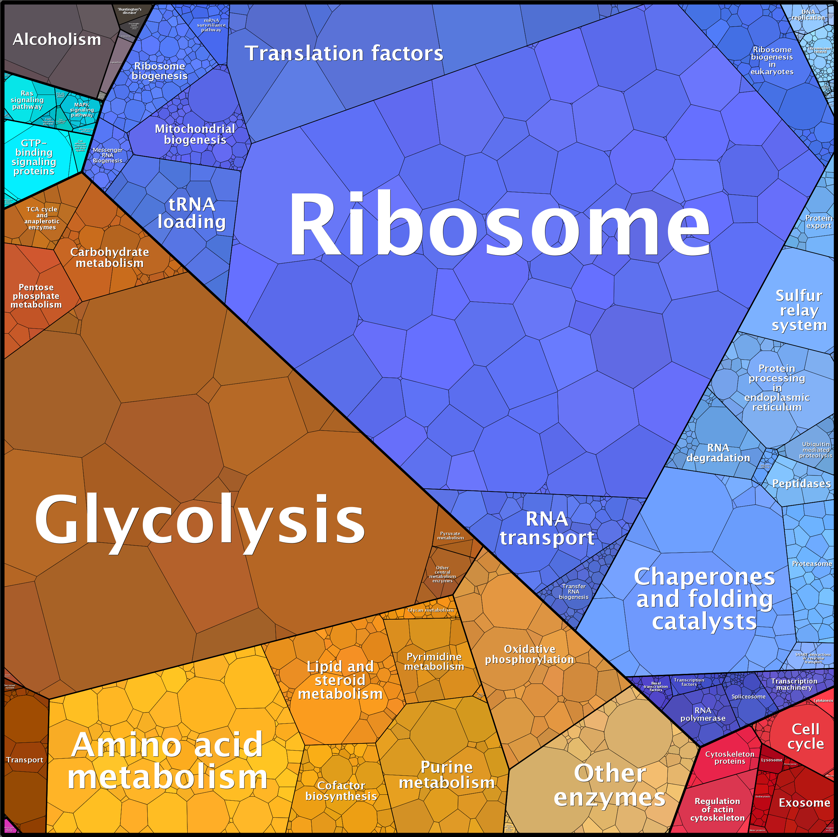
\includegraphics[width=.8\linewidth]{proteome2.png}
    \subcaption{タンパク質の発現量}
    \label{fig:prmap_pro}
  \end{minipage}
  \caption{プロテオーム(酵母)}
\end{figure}

ここで,酵母について遺伝子ごとに発現するタンパク質の機能を対応させると,図\ref{fig:prmap_gen}のようになる.
これより,タンパク質にはDNAの複製,転写,翻訳に関わるものと代謝や輸送に関わるものが同じくらいの種類あることが分かる.
ただし,この図では各遺伝子が同じ重みで表示されているため,遺伝子ごとに発現するタンパク質の量は反映されていない.
それを反映すると,図\ref{fig:prmap_pro}のようになる.
これより,発現するタンパク質の多くは翻訳(リボソーム)または解糖系に関わるといえる.
しかし,そのほかにも細胞周期やシグナル伝達に関わるものもいくらか存在している.
このように,発現量に偏りはあるものの,タンパク質の役割は様々である.

また,各タンパク質を発現量順に並べると,発現量の分布は順位の逆数に比例する(Zipf則に従う)ことが知られる.
これはHurusawa-Kanekoモデル(2003)によって説明されている.